\chapter{\IfLanguageName{dutch}{Stand van zaken}{State of the art}}
\label{ch:stand-van-zaken}

% Tip: Begin elk hoofdstuk met een paragraaf inleiding die beschrijft hoe
% dit hoofdstuk past binnen het geheel van de bachelorproef. Geef in het
% bijzonder aan wat de link is met het vorige en volgende hoofdstuk.

% Pas na deze inleidende paragraaf komt de eerste sectiehoofding.
\section{\IfLanguageName{dutch}{Global Positioning System (GPS)}{Global Positioning System (GPS)}}
\subsection{\IfLanguageName{dutch}{De werking van GPS}{How GPS works}}
\begin{figure}
	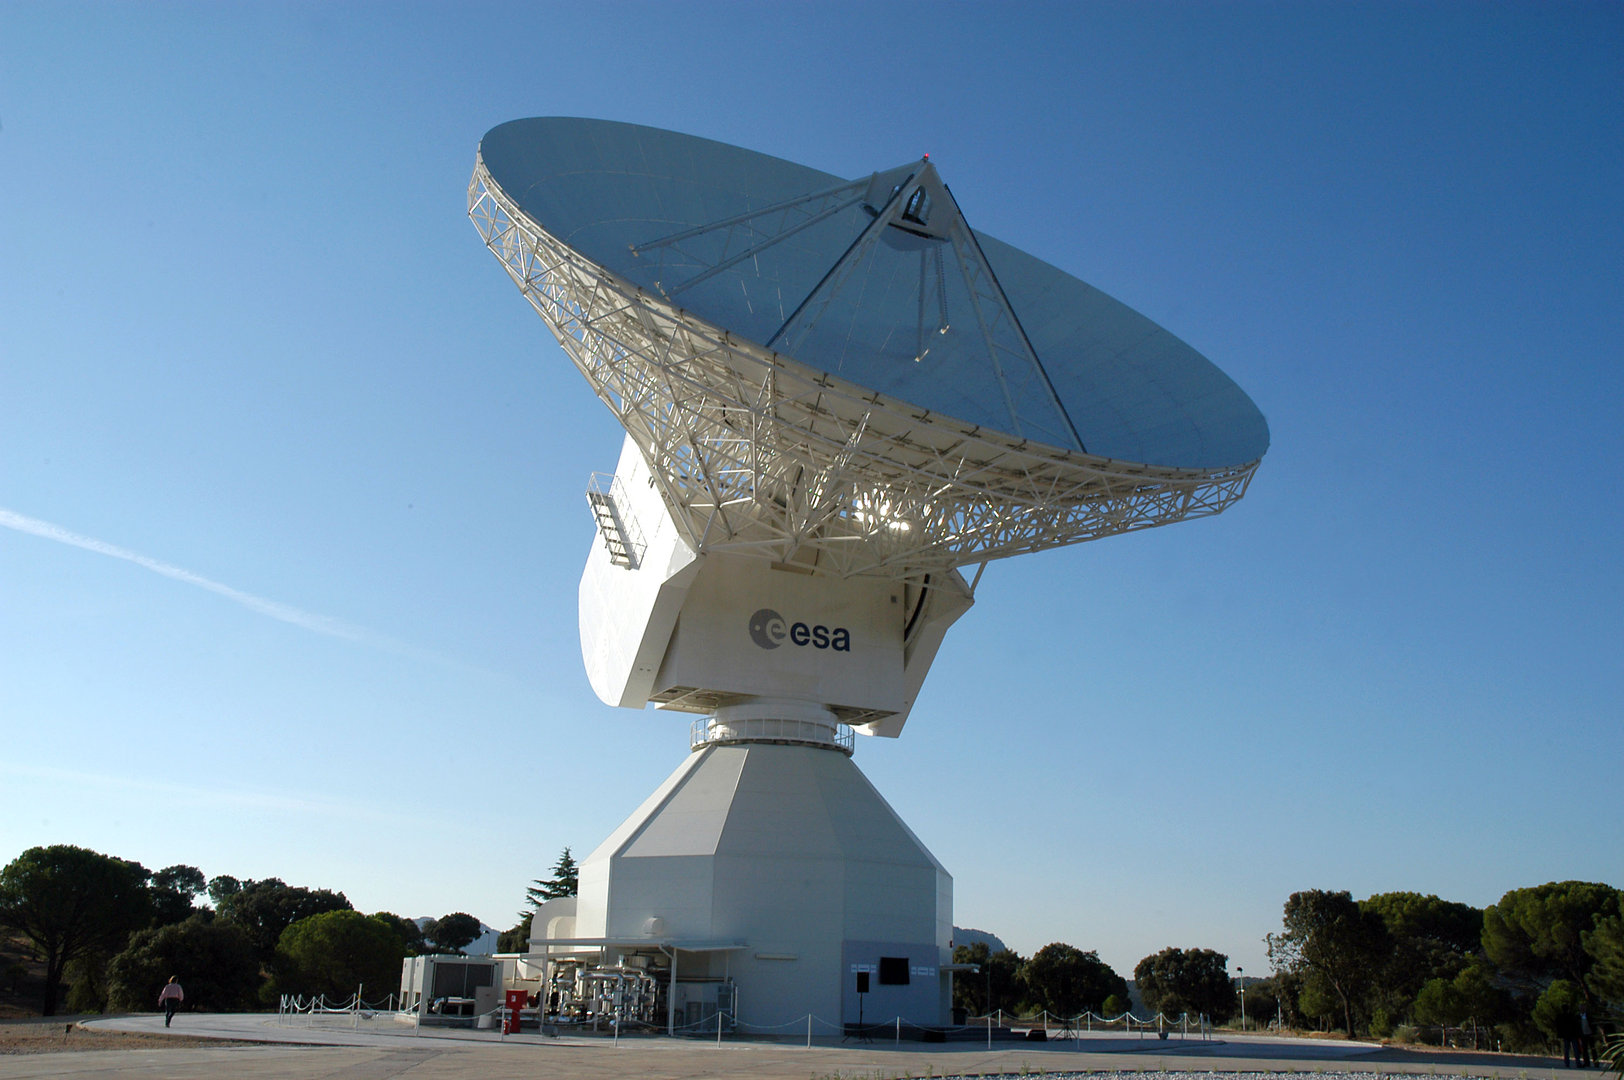
\includegraphics[width=\textwidth,height=\textheight,keepaspectratio]{groundstation.jpg}
	%https://www.google.com/url?sa=i&url=https%3A%2F%2Fwww.esa.int%2FAbout_Us%2FESAC%2FCebreros_ground_station&psig=AOvVaw3m4fRPzsoJEUD7uxKB9P8U&ust=1583062350499000&source=images&cd=vfe&ved=0CAMQjB1qFwoTCJD8uPrU9ucCFQAAAAAdAAAAABAD
	\caption{source:google}
	\label{fig:groundstation}
\end{figure}
\begin{figure}
	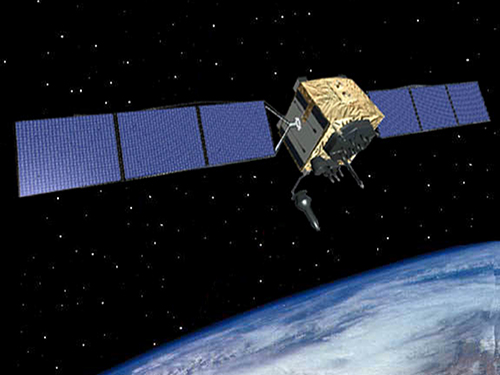
\includegraphics[width=\textwidth,height=\textheight,keepaspectratio]{satelliet.jpg}
	%https://www.google.com/url?sa=i&url=https%3A%2F%2Fspacenews.com%2F40530gps-2f-6-navigation-satellite-slated-to-launch-on-may-15%2F&psig=AOvVaw0tzOggmMim-1CxoYTRl1Ze&ust=1583062792344000&source=images&cd=vfe&ved=0CAMQjB1qFwoTCOD3jc3W9ucCFQAAAAAdAAAAABAD
	\caption{source:google}
	\label{fig:satelliet}
\end{figure}

Om een locatie te bepalen zijn er 3 zaken nodig:
\begin{itemize}
	\item Groundstations, deze zijn ontworpen voor buitenplanetaire draadloze communicatie. Ze communiceren door het ontvangen en verzenden van radiogolven met zeer hoge frequentie. (Zie figuur: \ref{fig:groundstation})
	\item Een satelliet, of ook vaak kunstmaan genoemd, is een object dat zich in een baan om een hemellichaam bevindt. \autocite{definitie_satelliet} (Zie figuur: \ref{fig:satelliet})
	\item GPS-ontvanger, dit ontvangt de elektromagnetische signalen van de satellieten.
\end{itemize}

De groundstations worden gebruikt om de locatie bij te houden van de GPS-satellieten. Deze stations worden niet gebruikt voor het bepalen van de huidige locatie van een gebruiker. 
\newline
\newline
De GPS-satellieten broadcasten een signaal uit die de afstand en tijd bevat. Deze tijd wordt bepaald aan de hand van een atomaire klok. Een regulaire klok kan na 6 weken een volledige milliseconde afwijken van de werkelijke tijd, wat zeer gevaarlijk is voor ruimteverkeer. Hierdoor maken satellieten gebruik van een ander type klok, de atomaire klok.Na 10 jaar wijkt een atomaire klok slechts een microseconde af, waardoor het veiliger is. Om deze afwijking te corrigeren worden er soms updates uitgevoerd. \autocite{atomic_clock}
\newline
Als de GPS-ontvangen de tijd en afstand uit het signaal heeft kunnen afleiden kan het aan de hand van triangulatie zijn locatie bepalen. (Zie figuur: \ref{fig:triangulatie})
Er wordt per satelliet een radius bepaald en er wordt gekeken naar de overlapping van drie satellieten. Na deze overlapping blijven er nog twee punten over waar de GPS-ontvanger zich mogelijks bevindt. Hiervoor is de vierde satelliet nodig. Deze laatste satelliet sluit een van de twee mogelijke locaties uit, waardoor de locatie van de GPS-ontvanger juist bepaald wordt (de juiste locatie kan afwijken van de realiteit, tabel \ref{tab:GNSS-vergelijking}). 

\begin{figure}
	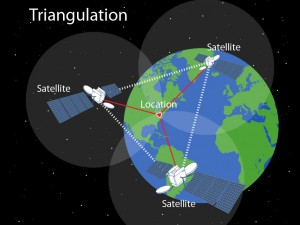
\includegraphics[width=\textwidth,height=\textheight,keepaspectratio]{triangulatie.jpg}
	%https://www.google.com/url?sa=i&url=https%3A%2F%2Fcommunicatiekc.com%2Ftriangulatie%2F&psig=AOvVaw3yrDqiAvEq65KAYiid2aw6&ust=1583063314296000&source=images&cd=vfe&ved=0CAMQjB1qFwoTCKCi68bY9ucCFQAAAAAdAAAAABAD
	\caption{source:google}
	\label{fig:triangulatie}
\end{figure} 
\pagebreak
\subsection{\IfLanguageName{dutch}{Global Navigation Satellite Systems (GNSS)}{Global Navigation Satellite Systems (GNSS)}}
Als we spreken over het bepalen van onze locatie, gebruiken we altijd de term 'GPS'. Toch klopt dit niet helemaal, want er bestaan veel meer technologieën en systemen die hierbij helpen. Iedere technologie wordt verder besproken in dit hoofdstuk.
\newline
Het 'Global Positioning System' is een ruimte gebaseerd radio navigatie systeem dat eigendom is van Amerika en bestuurd wordt door de 'United States Air Force' (USAF). Officieel heet dit systeem 'Navigation Satellite Time And Ranging' (NAVSTAR). De allereerste versie werd gelanceerd in 1978 en in 1995 operationeel verklaard. GPS is instaat om een ongelimiteerde limiet van gebruikers met een GPS-ontvanger te voorzien van hun locatie op ieder moment van de dag, onafhankelijk van het weer en over de hele wereld. \autocite{gps}
\newline
Naast NAVSTAR bestaat er ook:
\begin{itemize}
	\item Galileo, beheerd door de Europese Unie (EU).
	\item Globalnaya navigatsionnaya sputnikovaya sistema (GLONASS), beheerd door Rusland.
	\item BeiDou Navigation Satellite System (BDS), beheerd door China, ook Compass genoemd.
	\item Indian Regional Navigation Satellite System (IRNSS/NavIC), beheerd door India.
	\item Quasi-Zenith Satellite System (QZSS), beheerd door Japan
\end{itemize}

Er zijn verschillen tussen tussen deze Global Navigation Satellite Systems, namelijk de accuraatheid en het aantal satellieten. Ook zijn QZSS en IRNSS niet bedoeld als globale GPS-systemen. (Zie tabel:\ref{tab:GNSS-vergelijking})
\begin{table}[]
	\begin{tabular}{lll}
		Systeem & Aantal satellieten (actief) & Nauwkeurigheid                                                                        \\
				BDS     & 35                          & 3.6 meter                                                                      \\
		NAVSTAR & 31                          & 3-5 meter                                                                             \\
		GLONASS & 24+                         & 4-10 meter                                                                            \\
		Galileo & 24+                         & 20-50 centimeter                                                                      \\
		IRNSS   & 7                           & \textless 10 meter over India en \textgreater{}20 meter over de Indische Oceaan regio \\
		QZSS    & 7                           & 1 - 0,01 meter                                                                       
	\end{tabular}
\label{tab:GNSS-vergelijking}
\caption{tabel die een vergelijking geeft van alle Global Navigation Satellite Systems}
\autocite{gnss}
\end{table}
\newline
De reden voor het bestaan van deze verschillende systemen is van politieke aard. Zo wou de Europese Unie en Rusland onafhankelijk worden van Amerika (NAVSTAR). 
\section{Verschillende GPS-technologieën}
\subsection{\IfLanguageName{dutch}{Standard Positioning Service (SPS)}{Standard Positioning Service (SPS)}}
De 'Standard Positioning Service' (SPS) is een positionerings- en timingdienst die signalen broadcast op de GPS L1 frequentie. Deze frequentie, die gebruikt wordt door alle NAVSTAR GPS-satellieten, zorgt ervoor dat GPS vrij te gebruiken is voor iedereen. \autocite{gps}
\newline
Deze vorm van GPS is vrij accuraat, maar presteert minder in vergelijking met het 'Precision Positioning Service'. 
\subsection{\IfLanguageName{dutch}{Precision Positioning Service (PPS)}{Precision Positioning Service (PPS)}}
De 'Precision Positioning Service' (PPS) is een  positionerings- en timingdienst die signalen broadcast op de GPS L1 en L2 frequenties. Het functioneert hetzelfde als SPS, maar hierbij wordt er ook gebruik gemaakt van een precisie code (P) die alleen beschikbaar is voor geautoriseerde gebruikers. Hiermee wordt voornamelijk het Amerikaans leger en zijn allianties bedoeld. \autocite{pps} Voor september 2007 werd er gebruik gemaakt van 'Selective Availability' (SA). Zo kon het leger van Amerika de accuraatheid bewust degraderen voor veiligheidsredenen. De nieuwere GPS III satellieten zouden niet meer uitgerust zijn met de SA functie. 
\newline
Deze service wordt voor de proof of concept door voor de hand liggende redenen uitgesloten.
\subsection{\IfLanguageName{dutch}{Differential Global Positioning System (DGPS)}{Differential Global Positioning System (DGPS)}}
Differential Global Positioning System (DGPS) verbeterd de accuraatheid van GPS. Dit systeem maakt gebruik van correctie technieken. Deze technieken kunnen real-time gebeuren, maar ook na het bepalen van de locatie. DGPS vereist een GPS-ontvanger (referentie station) wiens locatie gekend is. De referentie gaat zijn locatie herberekenen en berekend het verschil tussen de gekende locatie en de berekende locatie. Het verschil wordt als volgt toegepast op de GPS-ontvanger wiens locatie we nog niet kenden. Deze techniek resulteert in een betere locatiebepaling voor de tweede GPS-ontvanger. \autocite{dgps} (Zie figuur:\ref{fig:dgps})
\begin{figure}
	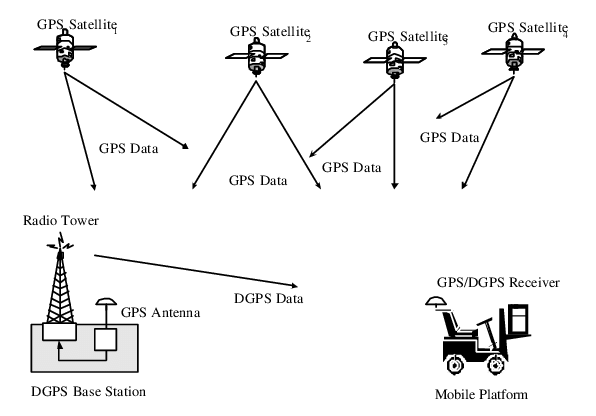
\includegraphics[width=\textwidth,height=\textheight,keepaspectratio]{dgps.png}
		%https://www.google.com/url?sa=i&url=https%3A%2F%2Fwww.researchgate.net%2Ffigure%2FComponents-of-a-DGPS-System_fig1_252064818&psig=AOvVaw07YsVmaU9ifoTgAxmkFPSb&ust=1583073831676000&source=images&cd=vfe&ved=0CAMQjB1qFwoTCPCjlt7_9ucCFQAAAAAdAAAAABAD
	\caption{source:google}
	\label{fig:dgps}
\end{figure}
\newline
De 'Flemish Positioning Service' (FLEPOS) maakt ook gebruik van deze techniek. De FLEPOS 3.0-netwerk bestaat momenteel uit 45 GNSS referentiestations, waarvan 33 referentiestations in eigen beheer uitbaat. Het gebruik hiervan is gratis indien de aanvraag voor een abonnement is goedgekeurd. In loop van deze bachelorproef zal de proof of concept proberen gebruik maken van FLEPOS 3.0 voor betere locatiebepalingen. 
\subsection{\IfLanguageName{dutch}{Wide Area Augmentation System (WAAS)}{Wide Area Augmentation System (WAAS)}}
'Wide Area Augmentation System' (WAAS) maakt gebruik van ground stations en GEO-satellieten, waardoor het in staat is om dezelfde correctie techniek als DGPS te gebruiken. \autocite{waas} Het gebruik van dit systeem is alleen mogelijk in Noord-Amerika, waardoor dit niet verder behandeld wordt in deze bachelorproef. 

\subsection{\IfLanguageName{dutch}{Assisted Global Positioning System (A-GPS)}{Assisted Global Positioning System (A-GPS)}}
Een GPS-toestel kan er enkele minuten over doen om je locatie te bepalen. Deze verloren tijd heet 'Time To First Fix' (TTFF). De duur van deze TTFF hangt af van je locatie en storing. Een open veld zal een kleinere TTFF hebben dan een stad. Assisted Global Positioning (AGPS/A-GPS/aGPS) verkleint de TTFF. 
\newline
Gsm masten hebben GPS-ontvangers die voortdurend informatie van GPS-satellieten verzamelen. Op deze informatie worden allerlei bewerkingen uitgevoerd en als volgt opgeslagen in een database. Dit heeft enkele voordelen voor de gsm die zijn locatie probeert te bepalen:
\begin{itemize}
	\item Snellere locatie bepaling.
	\item Minder computerkracht nodig.
	\item Minder batterijverbruik.
	\item Mogelijkheid om de locatie indoor te bepalen.
\end{itemize} 
Andere voordelen zijn:
\begin{itemize}
	\item Hoge accuraatheid (5-50 meter).
	\item Slechts twee waarneembare GPS-satellieten nodig.
\end{itemize}
Zoals je kan merken is de accuraatheid minder goed dan het zelf bepalen van de locatie (Zie: \ref{tab:GNSS-vergelijking}). Er zullen field tests en metingen worden uitgevoerd om deze stellingen te controleren. \autocite{agps}
\subsection{\IfLanguageName{dutch}{Advanced Mobile Location (AML)}{Advanced Mobile Location (AML)}}
Tot nu toe was er nog geen enkele techniek die de exacte locatie kon bepalen. 'Advanced Mobile Location' (AML) is de nieuwste (opensource) techniek die hiervoor een oplossing biedt. Het maakt gebruik van:
\begin{itemize}
	\item Wifi
	\item SMS
	\item GNSS
\end{itemize}
Door gebruik te maken van bovenstaande positioneringstechnieken is het de meest accurate en tegelijkertijd de traagste methode van alle besproken methodes. 
\newline
Deze methode wordt gebruikt bij noodtelfoon oproepen. Bij het begin van het bellen wordt er eerst gekeken of de Wifi en GPS aanstaat. Als de 'battery check' positief is, worden deze services aangezet indien ze nog niet aanstonden. 
\newline
AML gaat parallel zijn locatie proberen bepalen aan de hand van wifi, SMS en GNSS, zodat het zo min mogelijk tijd verliest om de beller te lokaliseren. De lokatie bepaling gebeurd aan de hand van een geprioritiseerde rij. Indien GNSS als eerste de lokatie kan bepalen wordt dit als eerst verzonden naar de hulpdiensten. 
Als tweede optie wordt de lokatie bepaald met behulp van wifi. Hierbij wordt de locatie gebaseerd op wifi 'Service Set Identifiers' (SSIDs) of MAC-adressen van access points waarmee de gsm verbonden is. Als laatste optie wordt de cell ID verstuurd van de mast waarmee de beller verbonden is. Indien men geen lokatie kan bepalen, wordt er een SMS verstuurd dat alle positioneringstechnieken (wifi, GNSS, cell ID) gefaald hebben.
\newline
Sinds Januari 2020 zijn er slechts 19 landen wereldwijd die AML implementeren. AML kan alleen gebruikt worden bij het bellen van het noodnummer, waardoor dit geen optie is voor de proof of concept. \autocite{aml}

\section{\IfLanguageName{dutch}{Ongunstige omstandigheden}{Unfavorable circumstances}}
\subsection{\IfLanguageName{dutch}{Water}{Water}}
\subsection{\IfLanguageName{dutch}{Sneeuw}{Snow}}

\section{\IfLanguageName{dutch}{Toestellen}{Devices}}
\subsection{\IfLanguageName{dutch}{Raspberry Pi}{Raspberry Pi}}
\subsection{\IfLanguageName{dutch}{Arduino}{Arduino}}